\documentclass[10pt,twocolumn]{article}
\usepackage{amsmath}
\usepackage{amsfonts}
\usepackage{amssymb}
\usepackage{graphicx}
\usepackage{cite}

\newcommand{\argmax}{\operatornamewithlimits{argmax}}
\newcommand{\argmin}{\operatornamewithlimits{argmin}}

\title{Handwritten Digit Classification on Textured Backgrounds}
\author{Ian Forbes, Xinchi Chen, Niladri Mohanty\\ Team: Mr. Pinks}
\begin{document}
\twocolumn[
\maketitle
\section{abstract}
We attempt to classify images of handwritten digits written on various textured backgrounds. Using a training set of 50000 $48 \times 48$ images we evaluate the performance of several popular machine learning algorithms including Naive Bayes, Fully Connected Feed Forward Neural networks, Support Vector Machines, and Convolutional Neural networks.
\\
\\
]
\section{Introduction}
Recently character recognition technology has been used in document analysis and recognition community due to the increasing demand of converting an enormous amounts of printed or handwritten information to a digital format. Application of optical character recognition (OCR) in converting historical, technical, and economic printed documents into digital form. There are some successful implementation of optical character recognition used the in digitization of handwritten documents. This field is quite challenging due to the high variability produced by noise, different handwriting styles, and image size and quality. Real world applications like bank cheque processing counts for handwriting variability\cite {diem2013icdar}. Also new handwritten digit dataset "CVL dataset" was released \cite {liu2003handwritten}. 

A fast and effective character recognition system required to solve the handwriting recognition problems such as bank cheque, automatic form processing or postal mail sorting. It is necessary to highlight that not only high speed but an accurate system is needed for classification process in real time environments. The main problem in recognizing character is variability. The same class character can be written in different sizes and orientation angles.

For improving the performance in recognition problems, image is divided into local regions \cite {lazebnik2006beyond}. This method is known as image zoning and highly successful in computer vision field\cite {ciresan2012multi}.

Recently Convolutional Neural Networks have given the best accuracy (99.73\%) on the MNIST dataset. Ciseran et al. expanded the training and testing dataset to including elastic distortions. Research have proven that negligence of distortion results into low accuracy rates \cite {gil2014handwritten}.
\section{Preprocessing}
We tried many different preprocessing methods in attempt to reduce image noise, sharpen the appearance of the target digit, and most importantly improve our algorithms' accuracy. The first and most basic of theses methods was to normalize all of the images to a $[0,1]$ scale. The reason for this decision was that while browsing through the images we noticed that many were mostly gray with very little black or white. We believed that by normalizing the images there would be more contrast between the digit and the background which would make it easier to identify the digit. While normalization proved promising in validation, increasing our validation accuracy by roughly 1\%, our actual Kaggle submissions scored lower than the un-normalized submission.

Another basic method to reduce noise from a signal is to average it across many samples.  We tried to average all images from the same class to get rid of noise. However as the noise (texture) is random, we found it was not a successful way to reduce the noise.

Another method we tried was image sharpening. Image sharpening works by subtracting a blurred copy of the image from a weighted version of the original image. The final sharpened image in our case was create by the formula: \[\text{sharpened} = 1.5 \cdot \text{original} - 0.5 \cdot \text{blurred}\]
Unfortunately this method showed no improvement over the non-sharpened images.

We also tried edge detection via the Laplacian operator $\Delta f$ (shown below left) which is the sum of the second derivatives. In order to calculate the the Laplacian the original image is convolved with the image filter (kernel)  below (right).
\[\Delta f = \frac{\partial^2 f}{\partial x^2} + \frac{\partial^2 f}{\partial y^2}
\qquad
\begin{bmatrix}
0 & 1 & 0 \\
1 & -4 & 1 \\
0 & 1 & 0
\end{bmatrix}
\]
This operation finds areas of the image where image intensity changes rapidly. The intuition being that fast changes in image intensity indicate edges. The problem with this approach however is that the image data becomes very sparse as the majority of the images tends to zero since there is little variation in much of the image. In order to remedy this we attempted to dilate the edges by one pixel. While this worked for images with smooth backgrounds it often caused those with noisy or rough backgrounds to become completely white since the background texture was also dilated. This method therefore reduced the performance of our algorithms.

In additional to applying various image filters we also attempted to increase the amount amount of data available us by adding rotated copies of the original data to our dataset. Since the digits from the original test were rotated at random we believed this would increase the amount to usable data and therefore our test results. This proved to not be an effective methods as it significantly reduced performance.

The Median filter can also be used to filter the noise. Again, it did not yield any considerable differences than raw images. Therefore, we did not focused on this technique of preprocessing.

After trying these various methods we found that the raw image data performed the best.
\section{Feature Selection}
For the majority of our algorithms we used the raw pixel values. However we also tried some  more complex methods to extract features from the image data.

Blockwise histograms of local orientations is one method of feature selection that can be used to recognize objects\cite{Maji09fastand}. This is called Pyramid Histogram of Oriented Gradients (PHOG). Each pixel in the image is assigned an orientation and magnitude based on the local gradient. Following this histograms are constructed by aggregating the pixel responses within cells of various sizes. The grayscale input image is then convolved with filters which respond to horizontal and vertical gradients from which the magnitude and orientation is computed. The orientation could be signed (0-360) or unsigned (0-180). The signed gradient distinguishes between black to white and white to black transitions which might be useful for digits. PHOG features are discussed further in  section 5.3.
\section{Algorithms}
\subsection{Naive Bayes}
Naive Bayes is a basic machine learning algorithm based on Bayes rule that can be used for multiclass classification. It uses Bayes rule along with the assumption that all features are conditionally independent given the class. The decision rule for Bayes rule is given by:
\[ \argmax_c \Pr(C = c) \prod_{i=0}^{n} \Pr(F_i = f_i | C = c)\]
We used a variant of Naive Bayes called Multinomial Naive Bayes. This method creates a Multinomial probability distribution for each of the features given the class. Mathematically speaking we estimate the distribution $\Pr(F_i = f_i | C = c)$ over each of the features $f \in F$ give the class equals $c$ using our training data. Then we use the decision rule to find the class $c$ which maximizes this probability when classifying a test example.

In order to model the probability distributions of $\Pr(F_i = f_i | C = c)$ as a multinomial distributions we needed to discretize the the continuous $[0,1]$ values present in the images to integer values. In order to do this we created a histogram with $B$ bins where intervals of size $1/B$ from $[0,1]$ were mapped to each bin. For example in the case where $B = 2$, pixels with intensity in the range $[0,0.5]$ would be mapped into bin 1 whereas pixels with intensity in $(0,5,1.0]$ would be mapped to bin 2. This essentially binarizes the image.

Ideally the number of bins $B$ would be extremely large so that pixels would be assigned to bins with very fine precision. The goal being to exactly replicate continuous distribution perfectly. However this would require near infinite data to construct. Because of this we need to select $B$ very carefully. In order to select $B$ we performed 10 fold cross validation. We found $B=27$ to be the optimal value scoring 37.048\%. Our cross validation results for $B$ are shown in figure \ref{bins}.
\begin{figure}
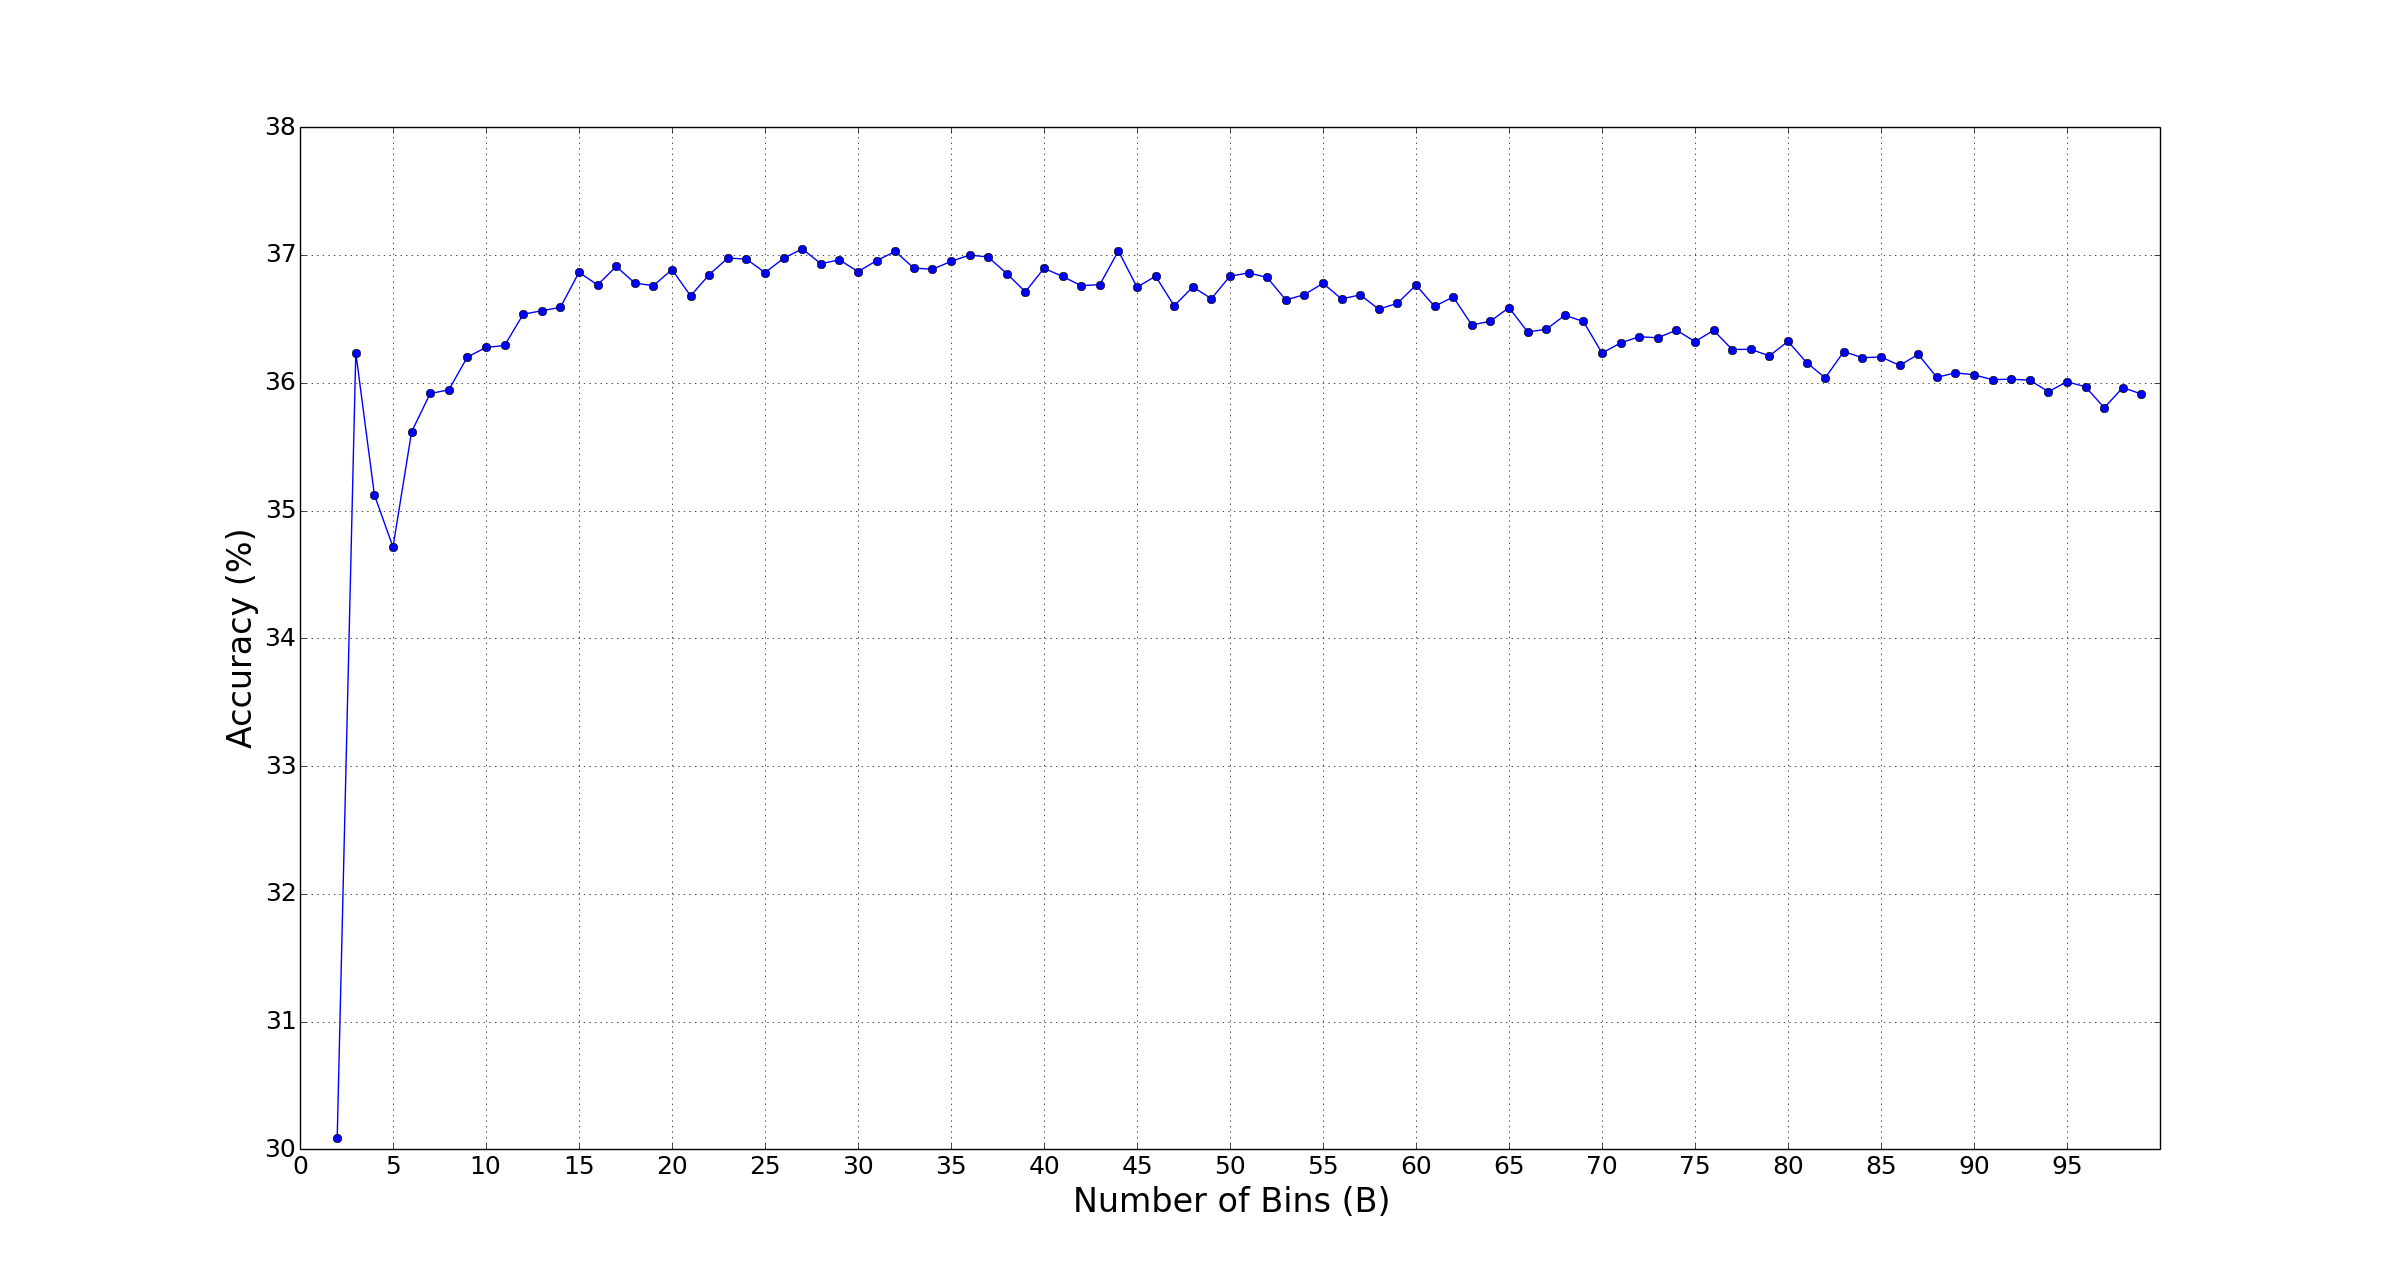
\includegraphics[trim=150 40 150 50,clip=true,width=0.5\textwidth]{./figure_1.png}
\caption{Naive Bayes Accuracy as a function of the number of bins $B$. The best value of $B$ was found to be 27 with accuracy 37.048\%.}
\label{bins}
\end{figure}
\subsection{Neural Network}
In the second part, we implemented a fully connected feedforward neural network, trained by back-propagation (abbreviated as “BPNN” in the following content). This part is programmed using python 2.7.8 with the Numpy extension. Numpy is a fundamental package for scientific computing with python, and is especially powerful at matrix calculations and transformation\cite{numpy}.

We used the raw image as our input data with no preprocessing as it showed to be ineffective with the other algorithms.

As the output result of an active (sigmoid function) is in the interval [0,1], we normalize the training output also to this interval.
\begin{figure}
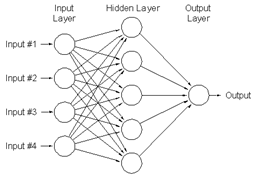
\includegraphics[width=0.5\textwidth]{./image.png}
\caption{A prototypical Feed Forward Neural Network.}
\end{figure}
To implement the BPNN we first generated random weights for each of links between input layer, hidden layer and output layers. Next, we calculated the inner product of weights and input and put the result through the sigmoid function. This is the Feed Forward step. After we got the result from output layer, we compare it with the given training outputs. The difference between the two results is then used to adjust the weights during the backpropagation to hidden layer---output layer and input layer---hidden layer sequentially.

We runs the program until the error converges. Note that since we are starting with a random set of weight and threshold, it may take a series of trails to make the error converge to the desired value.

In order to find the optimal value from the number of neuron in the hidden layer and learning rate we used 5 fold cross-validation. The results of our validation step can be seen below. 
\\
\\
\begin{tabular}{|c|c|c|c|}
\hline
 \# Neurons $\diagdown$ LR & 0.3 & 0.5 & 0.8 \\ \hline
 8 & 17.75\% &  16.95\% & 13.38\% \\
 30 & 22.28\% & 25.24\% & 21.75\% \\
 50 & 21.67\% & 23.72\% & 21.53\% \\ \hline
\end{tabular}

From the above result, we can see that the learning rate and neuron numbers will significantly effect the networks performance.  From our simulation, it is observed that 30 hidden layer nods and learning rate=0.5 gives the best performance.

Theoretically, having too many hidden neurons will cause the network to over fit and therefore ibe incapable of generalization. In contrast, having too few neurons will make the system not described adequately. Also, the system will be less robust to damage.

\subsection{Support Vector Machine}
Support vector machines (SVMs) have shown to been a promising tool for data classification. The basic idea behind SVMs is to map data into a high dimensional space and find a separating hyperplane with the maximal margin.

A Combination of features and SVM is used to classify using SVM classifier \cite {chen2006combining}. In all cases, model selection was performed using a validation set. Linear SVM is used to classify test dataset. One vs all classification approach is used for multi class SVM classification. 50000 training samples are divided into 42000 training dataset and 8000 validation dataset for all the trials of SVM. For C = 0.1, linear SVM validation accuracy for PHOG features is 14.63\% and test dataset accuracy is 10.54\%.  When C is selected as 10, validation accuracy dropped to 10.89\%.

Linear SVM fails to classify test dataset by PHOG features. It can be inferred that PHOG features can not be used to classify data using linear separation.
SVM can also perform efficiently for datasets which are not linearly separated. For non-linear classification, it computes a new feature for every given example depending on proximity to landmarks. It is important to note that these landmarks are chosen to be equal to $x_i, i=1,…,m$. Given $x$, the new features are computed as-
\[f_i=\text{similarity}(x_i,l_i)\]
 
To test whether SVM is a good classifier for this kind of problem or not, we tried SVM with Gaussian kernel. The Gaussian kernel function is given below:

\[f_i=\exp\Big(\frac{-‖x-l_i ‖}{2\sigma^2 }\Big)\]

SVM classifier with gaussian kernel is tested with σ ranging from $10^-7$ to $1$ and C = 0.1 to $10^5$ \cite {larochelle2007empirical}. Gaussian kernel SVM results for different sigma and C is shown in table 1. 
\\
\\
\begin{tabular}{|c|c|c|c|}
\hline
$\sigma$ & C &	Validation & Test Accuracy \\
\hline
$10^{-7}$  & 0.1	& 31.52\%	& 26.78\% \\
$10^{-5}$	 & 10	& 32.61\%	& 29.82\% \\
$10^{-3}$	 & $10^3$ & 29.61\%	& 26.59\% \\
1        &$10^5$ & 	24.94\% & 	17.29\% \\
\hline
\end{tabular}
\\

Table 1. PHOG features gaussian SVM result
\\

The best accuracy by SVM is 32.61\% on validation dataset and 29.82\% on test dataset. We concluded that PHOG features are not best suited for this kind of problem where image is combined with lot of random textures. Although, Maji et. al. obtained very low percentage of error with the same features because their images were free from any noise.

We also tested SVMs both kernels for raw data. The accuracy for validation and test datasets are shown in table 2.
\\

\begin{tabular}{|c|c|c|}
\hline
Kernel & Validation accuracy & Test accuracy \\ \hline
Linear & 42.06\% & 39.48\% \\
Gaussian & 40.24\% & 39.21\% \\
\hline
\end{tabular}
\\

Table 2. Linear \& Gaussian kernel SVM result
\\

\subsection{Convolutional Neural Network}
While Convolutional Neural Networks (CNNs) have been around for many years it is only recently that they have become computational feasible to train. Using Graphics Processing Units (GPUs) researchers from the University of Toronto showed that not only can CNNs be made feasible to train but that they can also outperform many other state of the art image recognition methods\cite{imagenet}.

The structure of Convolution Neural Networks is inspired by the mammalian visual system. During the 1970's Hubel \& Weisel conducted a vast amount research on cats and monkeys in order to try to understand the biological vision systems of the brain\cite{hubel}. Their research showed that vision system, at least in the few first layers, was highly localized. This meant that neurons in higher layers of the visual system only accepted inputs from groups neurons with were receiving their input from the same area in the visual field. Convolutional Neural use this notion of locality when building their neurons. Where as Fully Connected NNs accept inputs from all other neurons CNNs attempt to model the biological vision system by taking locality into account in the first layers of the network. The locals layers are then feed into a Fully Connected NN at the end of the network to compute the final output. This has allowed CNNs to achieve remarkably good results in the area of image recognition since spacial locality is extremely important.
\subsubsection{Methodology}
In order to build our CNN we used the Caffe CNN framework\cite{jia2014caffe}. Caffe allows one to create a CNN using Google Protocol Buffers, a structured data definition language similar to XML and JSON. User can define the structure of the network including data input layers, convolution, pooling, and fully connected layers as well as output layers such as loss, argmax, and accuracy. Using Caffe one simply has to define the network no coding required. Caffe then compiles this definition file and builds the network from it.

We based our final network off of the LeNet architecture \cite{lecun-01a}. This architecture was recommend by the MNIST tutorial provided on Caffe website. Since our dataset is very similar to the MNIST dataset we believed this would be a good place to start. 

In order to train and validate the performance of our network we segmented the dataset into 5 parts. We used the first 4 segments (40000 images) to train network and the last segment (10000 images) to validate it. We did not perform cross validation as the cost of train the network was quite high. 
\subsubsection{Network Architecture}
Using the LeNet architecture as a our starting point we managed achieved achieve 86.7\% accuracy on the public Kaggle test set. By adding an additional convolutional and pooling layer we managed to increase this to 91.5\%. Next we increased the initial learning rate from 0.1 to 0.5 (a learning rate of 1 lead to NaN errors) in hopes that the previous network had fallen into a local minimum. After increasing the initial learning rate to 0.5 we scored 92.1\%. 

Adding a fourth layer posed a slight problem as each convolutional and pooling layer reduces the size original input of $48 \times 48$. In fact the output of the 3 layer network using 5,5,5 for kernels was a single scalar value. Because of this a fourth layer could not added using this scheme. In order to remedy this we had to reduce the kernel size, and therefore the rate of input size reduction in the proceeding layers. In the end the 4 layer network used 5,5,3,3 for its kernel sizes. Unfortunately the 4 layer network proved to be significantly worse than the 3 layer network, only scoring in the 75\% range. Because of this, and the fact that the extra layer increased the training time, we choose no to train any additional 4 layer networks.

A visualization of our final network can be viewed in the appendix.
\begin{figure}
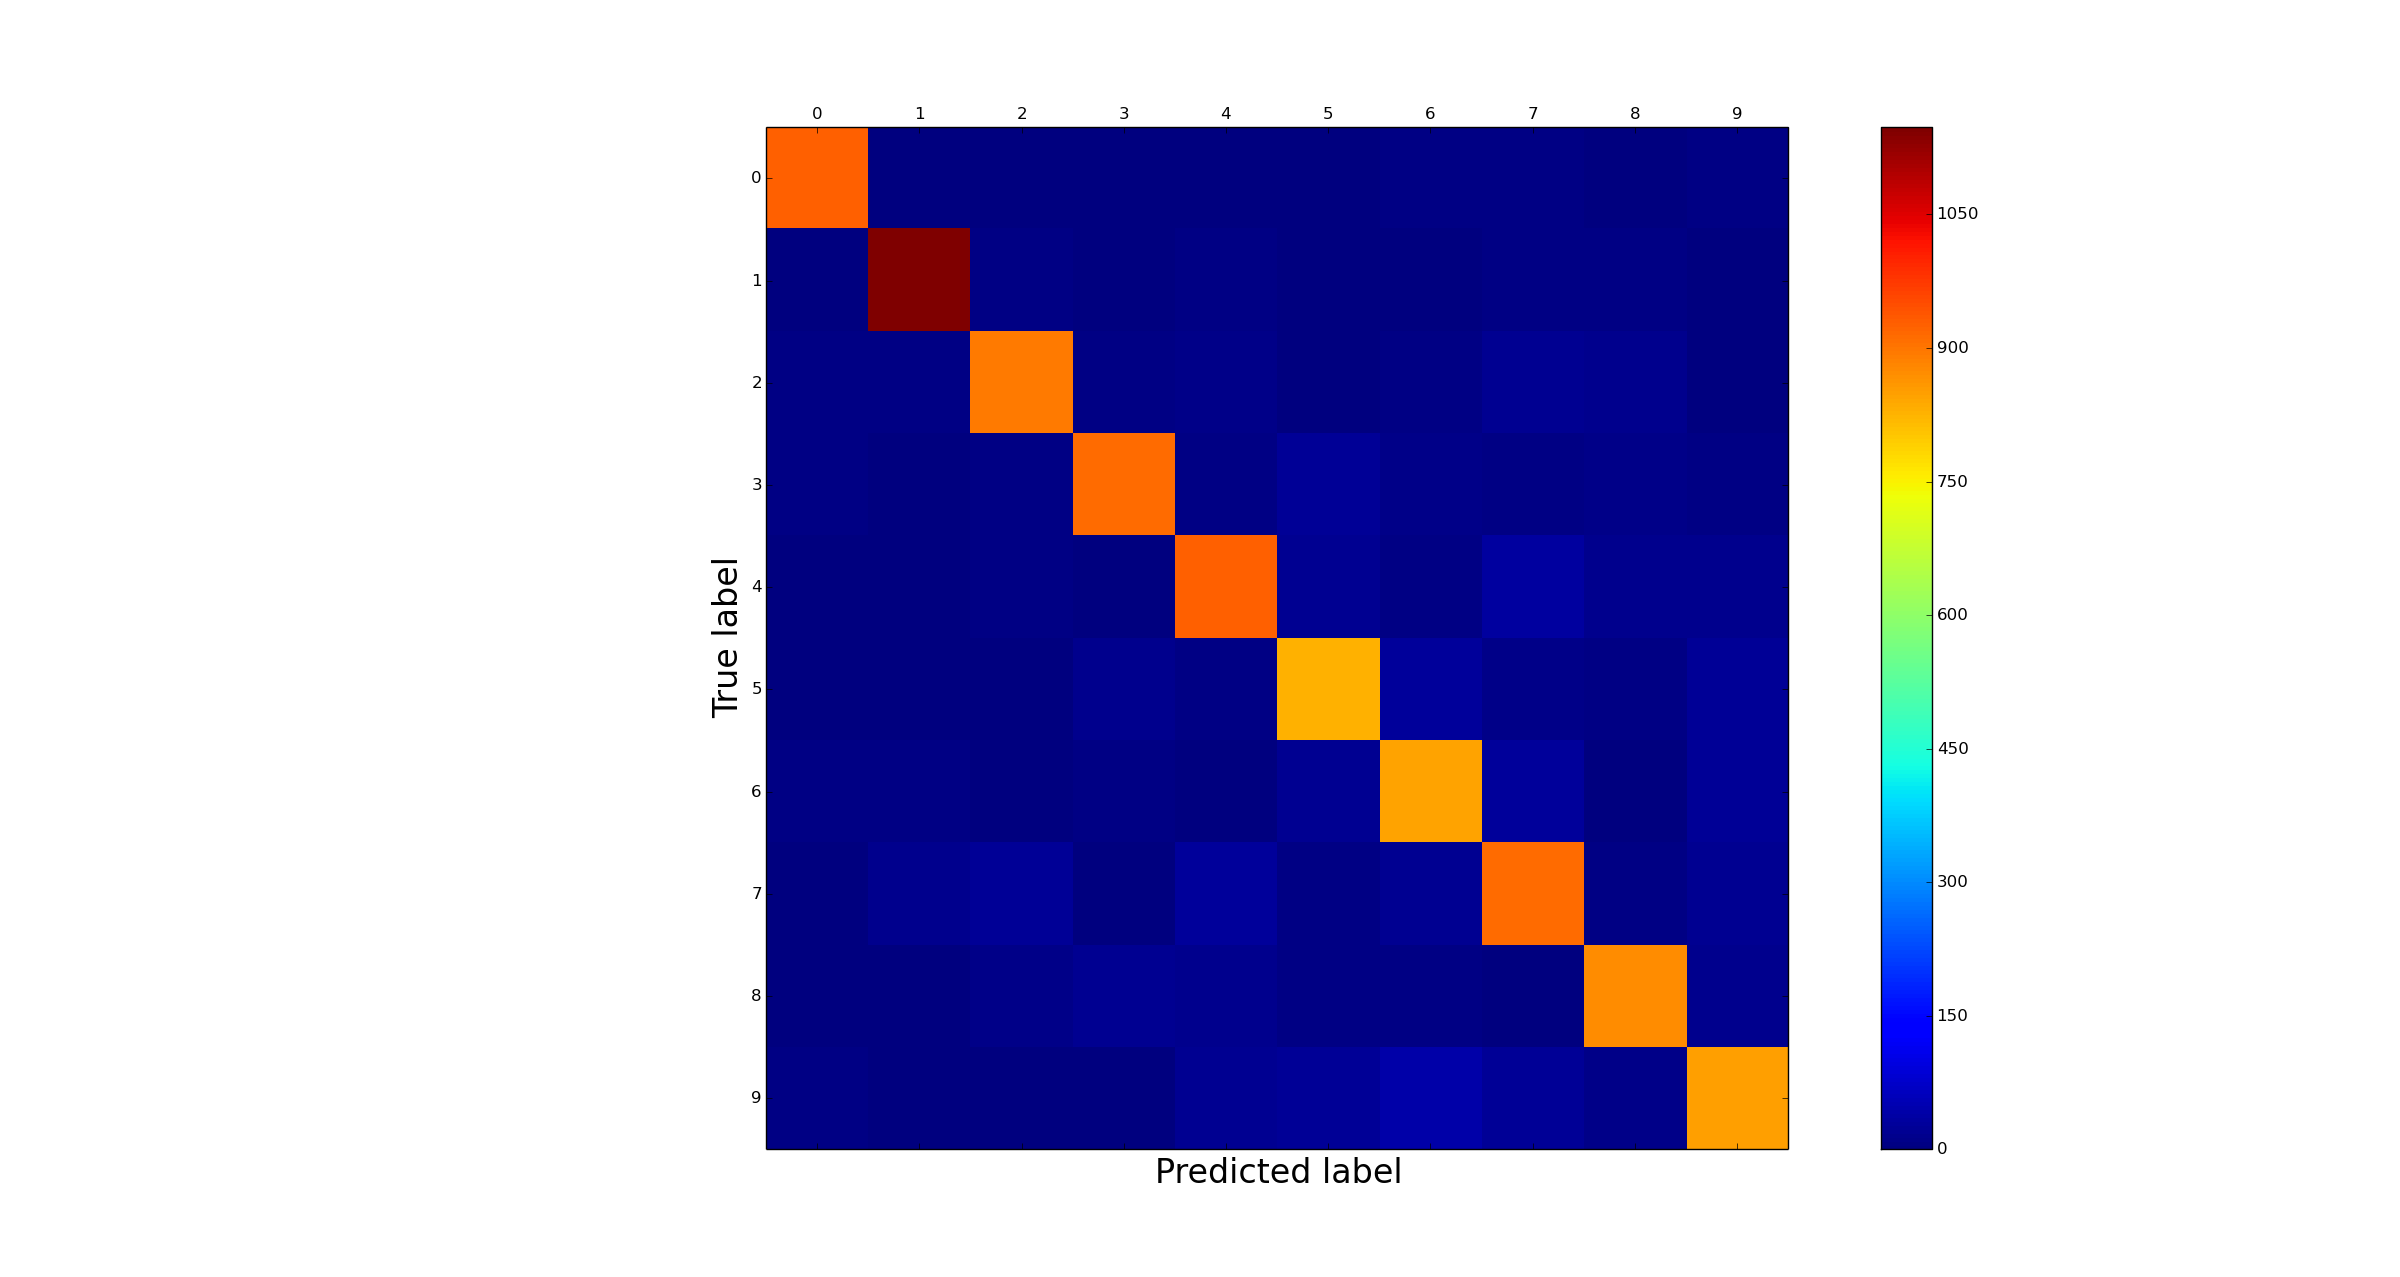
\includegraphics[trim=500 50 200 50,clip=true,width=0.5\textwidth]{./confusion.png}
\caption{Confusion Matrix for CNN. When training on all of the training data this network scored 92.6\% on the public Kaggle test set.}
\end{figure}
\subsubsection{GPU Training}
In order to train our network we used a single nVidia GTX 860m GPU with 2GB of memory. This allowed us to train and validate our networks to convergence in roughly 30 minutes. This allowed us to easily tune parameters and add or remove layers from the network in order to see their effect on the test score. We found that 10000 iterations was sufficient for the network to converge. In fact more iterations usually caused the networks performance to decrease slightly. For example 20000 iterations caused a reduction of $\sim 0.5\%$ on the public Kaggle test set. 

\section{Discussion}
We found that Naive Bayes did much better than expected. Naive Bayes' assumption that features are conditionally independent give then class is clearly a very bad assumption to make for image data since spatial locality of the data is very important. Naive Bayes independence assumption basically throws away this locality information. Regardless it was able to perform just as well as other algorithms such as SVM which usually preform better on other problems. 

BP neural networks have many advantages. First of all, BP neural networks can realized the mapping from input to outputs. Because of this strong non-linear mapping characteristic, BP is extremely suitable for solving problems with complex mechanisms. In other words, BP neural networks can be used even if users does not understand the solution. In contrast to many other traditional techniques, users must understand the inputs, the algorithms, and the outputs in great detail, to make the implementation work.

Secondly during the training process BP network will automatically learn to retrieve the `inner connection' between inputs and outputs, and apply this to learning the weights. Therefore, BP networks are highly self-learning and adaptive.

However, BP neural network also has some critical disadvantages. One of the most critical shortcomings for BP neural network is the “local minimum” issue. The traditional BPNN is an optimization to local search, and it solves complex non-linear by tweaking the weights gradually. However, this approach may bring the algorithm to a local minimum, and eventually leads to training failure. In addition to this BPNN is very sensitive to initial network weights. Initializing the network with different starting weight may greatly affect the convergence of BPNN. This is also the reason why different trials may give different convergence result.

Another disadvantage of BPNN is that it can take a large number of iterations to converge to the desired solution\cite{regression}. As BPNN uses gradient descent to explore a complex function, “serrated plot” is likely to happen during in this process. Therefore, BPNN is relatively low in computational efficiency. One potential solution to this is PNN\cite{prob}\cite{nn}.

Support Vector Machines using a linear kernel does clearly not give satisfactory results for raw features or PHOG features. It is evident that separating this dataset using linear decision boundary (either Naive bayes or Linear SVM) will result accuracy around 40\%. Even using Gaussian (RBF) kernel is not very effective. Because of this we concluded that SVM is not a suitable algorithm for image classification.

Convolutional Neural networks are the clear winner when it comes to image recognition. When coupled with GPUs this method is significantly better then all the other methods we explored. Since their introduction in 2012 nearly all teams competing in the ImageNet competition have switched to using CNNs and GPU training or some slight variation \cite{nvidia}.

\bibliographystyle{unsrt}
\bibliography{biblio.bib}
\section*{Appendix}
\begin{figure*}
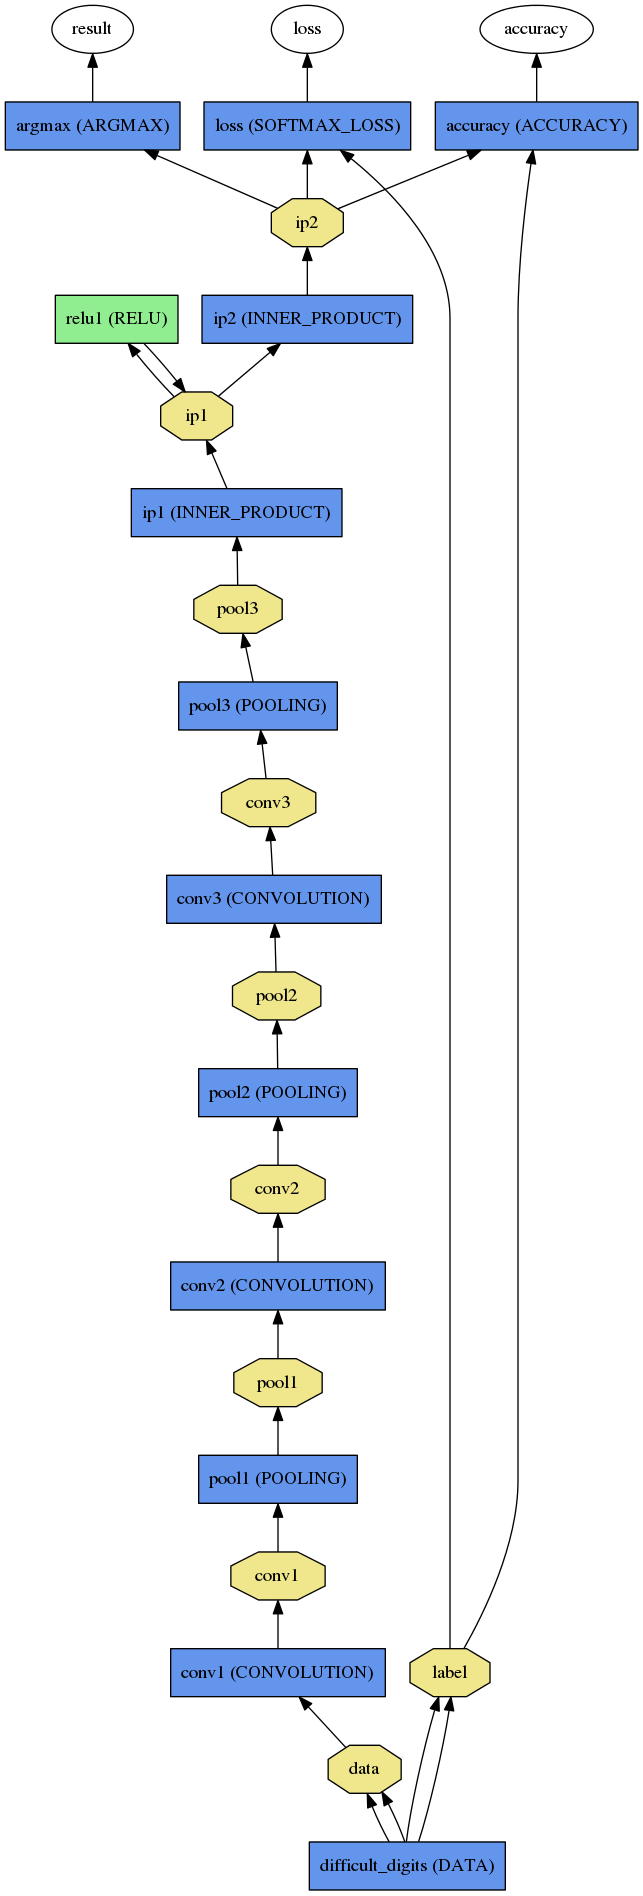
\includegraphics[scale=0.30]{./nn.png}
\caption{Visualization of our Convolutional Neural Network.}
\end{figure*}

\begin{figure*}
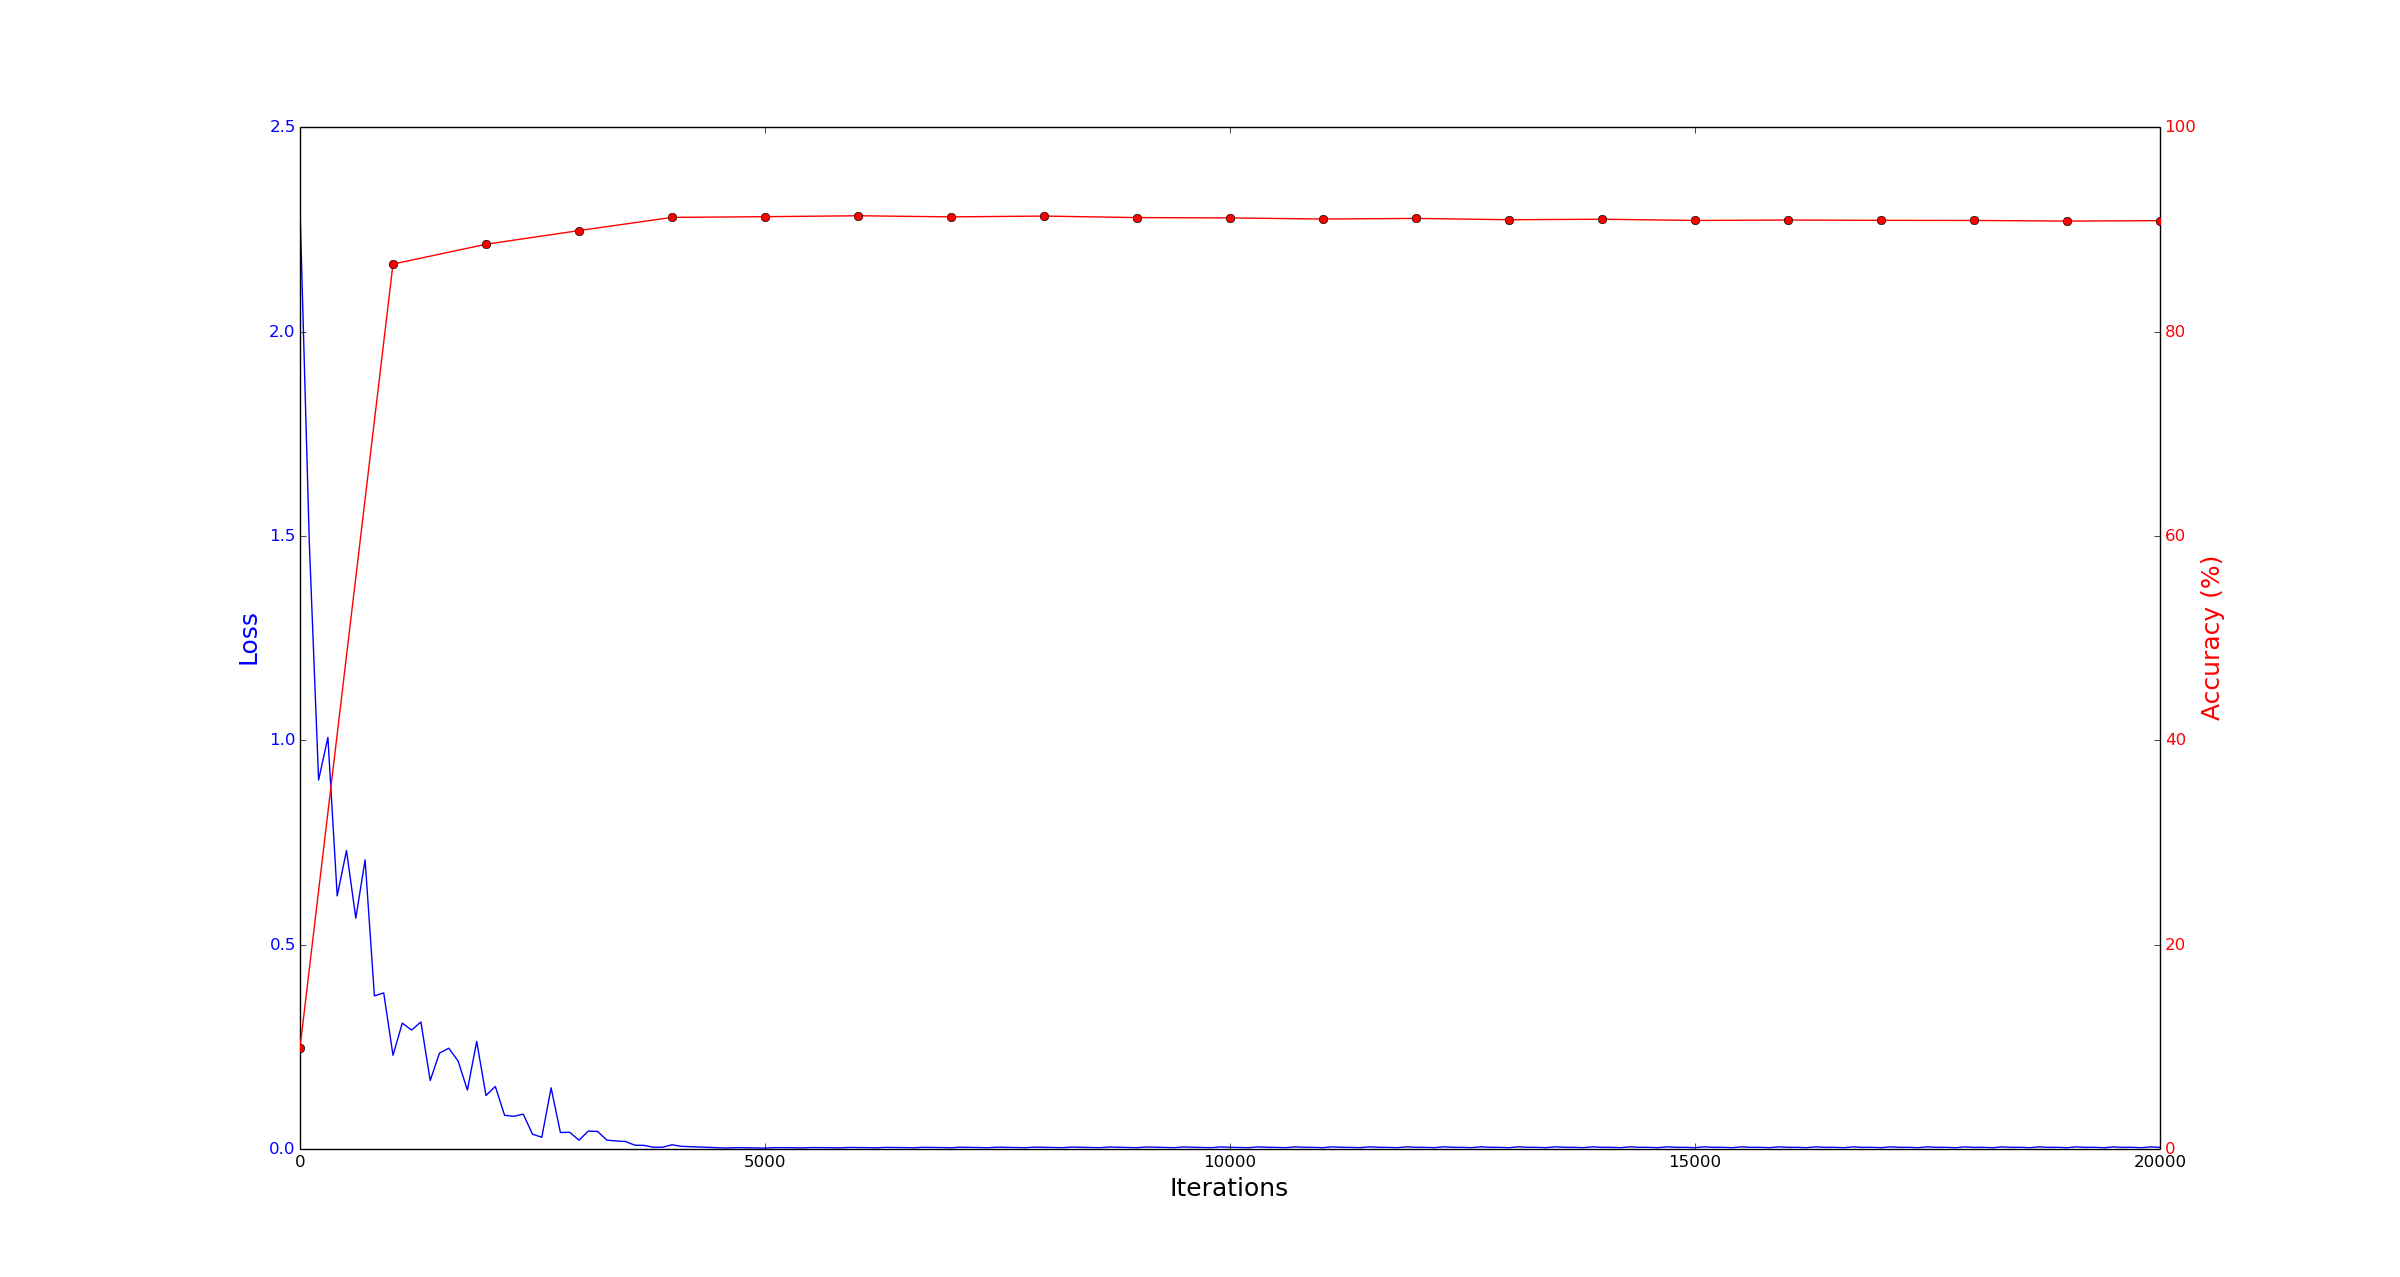
\includegraphics[trim=100 50 100 50,clip=true,scale=0.3]{./loss.png}
\end{figure*}
\end{document}
